\documentclass[answers,11pt]{exam}
\usepackage[utf8]{inputenc}
\usepackage[norsk]{babel}
\usepackage[T1]{fontenc}
% \renewcommand{\rmdefault}{cmss}  % times new roman font
\usepackage{verbatim,a4,amsmath}
\usepackage{epsfig,amssymb,array,delarray}
\usepackage{tabularx,enumerate,alltt,float}
\usepackage{rotating,wrapfig,amsmath}
\usepackage{longtable,color,boxedminipage}
\usepackage{graphicx,lscape,ulem}
\usepackage[most]{tcolorbox}
\parindent0mm

\usepackage[figurer/]{figurepath} 
\usepackage{here,hyperref}

\usepackage{listings}
\usepackage[framed,numbered,autolinebreaks,useliterate]{mcode}
\lstset{inputencoding=ansinew,
  literate=  {ø}{{\o}}1%
  {æ}{{\ae}}1%
  {å}{{\aa}}1%
  {Ø}{{\O}}1%
  {Æ}{{\AE}}1%
  {Å}{{\AA}}1%
}

\definecolor{darkgreen}{rgb}{0.0, 0.6, 0.0}

\textheight210mm
\textwidth145mm
\marginparsep0mm
\oddsidemargin10mm
\parskip 2mm plus 2mm minus 2mm % gir TeX litt fleksibilitet for sidebrekk

\lstset{language=Matlab,
  basicstyle = \tiny 
}

\begin{document}
\renewcommand{\solutiontitle}{\noindent\textbf{}\par\noindent}
\shadedsolutions
\renewcommand{\thequestion}{\alph{question})}
\renewcommand{\questionlabel}{\thequestion}
\renewcommand{\solutiontitle}{\noindent\textbf{Svar:}\par\noindent}

\renewcommand{\lstlistingname}{Kode}% Listing -> Kode
\renewcommand{\thepage}{\arabic{page}}
\cfoot{\thepage}

\pagestyle{headandfoot}
\runningheadrule       
\firstpageheader{}{}{}

\selectlanguage{norsk}
\setlength{\parskip}{0.5cm}


\vspace*{2cm}

\begin{center}
  {\Large \bf ELE130 Anvendt fysikk og matematikk i robotprogrammering}\\[2cm]
  \vspace*{2cm}
  {\LARGE \bf  Øving 3\\[5mm]
    Introduksjon til
    numerisk integrasjon,\\[1mm]
    numerisk derivasjon 
    og filtrering\footnote{Tilhørende
      filer: \fbox{\tt oving3\_skallfiler.zip} og {\LaTeX}-mal i \fbox{\tt oving3.zip}. }}
\end{center}

\vspace*{3cm}
\begin{tcolorbox}
  {\Large \bf  Levert av ....}
  
\end{tcolorbox}



\section*{Om øvingen og innleveringen}

\begin{boxedminipage}{\textwidth}
    \begin{itemize}
      \setlength\itemsep{0mm}
    \item For å bli kjent med prinsippet bak numerisk integrasjon,
      numerisk derivasjon og filtrering, 
      så er alle oppgavene i denne øvingen svært nyttige,
      og de vil fungere som et oppslagsverk for deg når du gjør senere
      øvinger.


  \item For å tilrettelegge for at du skal gjøre flest mulig oppgaver,
    så kan du laste ned og pakke opp \fbox{\tt oving3\_skallfiler.zip}.
    I denne zip-filen vil finne
    \begin{itemize}
    \item  skallfilen \fbox{\tt oving3\_skallfil.m}
      som inneholder uferdig kode for alle oppgavene i denne øvingen
    \item  skallfiler for alle funksjonene som du skal ferdigstille
    \item simulink-skallfilen \fbox{\tt oving3\_a\_m\_skallfil.slx}
      for oppgavene 3a) og 3m)
    \end{itemize}
    Mange av oppgavene virker kanskje omfattende, men svært
    mye av ``infrastruktur-koden'' er allerede
    gitt.

 \item   På tilsvarende måte som i øving 1 bør du bruke trikset
    med å først kommentere hele skriptet \fbox{\tt oving3\_skallfil.m}
    for deretter å ta bort
    kommentarene celle for celle. 

    \item {\bf Hensikten med   øvingen er du skal bruke
      oppgavene som et verktøy til å gi deg forståelse og innsikt for
      de forskjellige temaene/begrepene.}


  \item   {\color{red}  For å få øvingen godkjent må du minst
      gjøre følgende oppgaver:\\
      \fbox{b), d), e), f), h), i), j) }}

      \item   Oppgavene   \fbox{a), c), g), k), l), m), n) o) }  er
        også lærerike og nyttige, men frivillige. Dette er markert i toppteksten.

\item   {\color{red}  For å ta eksamen i emnet  ELE130 så må denne øving være
  godkjent. Husk at øvingene må leveres individuelt.}

  \item Basis for denne øvingen er
    {\color{blue} kapittel 7, 8 og 9} i kompendiet.

    \item På samme måte som i øving 1 og 2 finner du en {\LaTeX}-mal i filen 
    \fbox{\tt oving3.zip}.

  \end{itemize}
  \end{boxedminipage}

  
  



  




\begin{tcolorbox}[breakable, enhanced]
  \section*{Forskjellig {\LaTeX}-kode}
  Under er det gitt litt forskjellig kode som du kan kopiere inn i
svarene under de oppgavene du gjør. Husk bare på å oppdatere
bokmerkene til nye, unike navn, så slipper du feilreferering.

  \begin{itemize}
  \item    Resultatet fra scopet er vist i figur~\ref{fig:3a}. 
    
    \begin{figure}[H]
      \centering
      \hspace*{0mm}\scalebox{0.35}{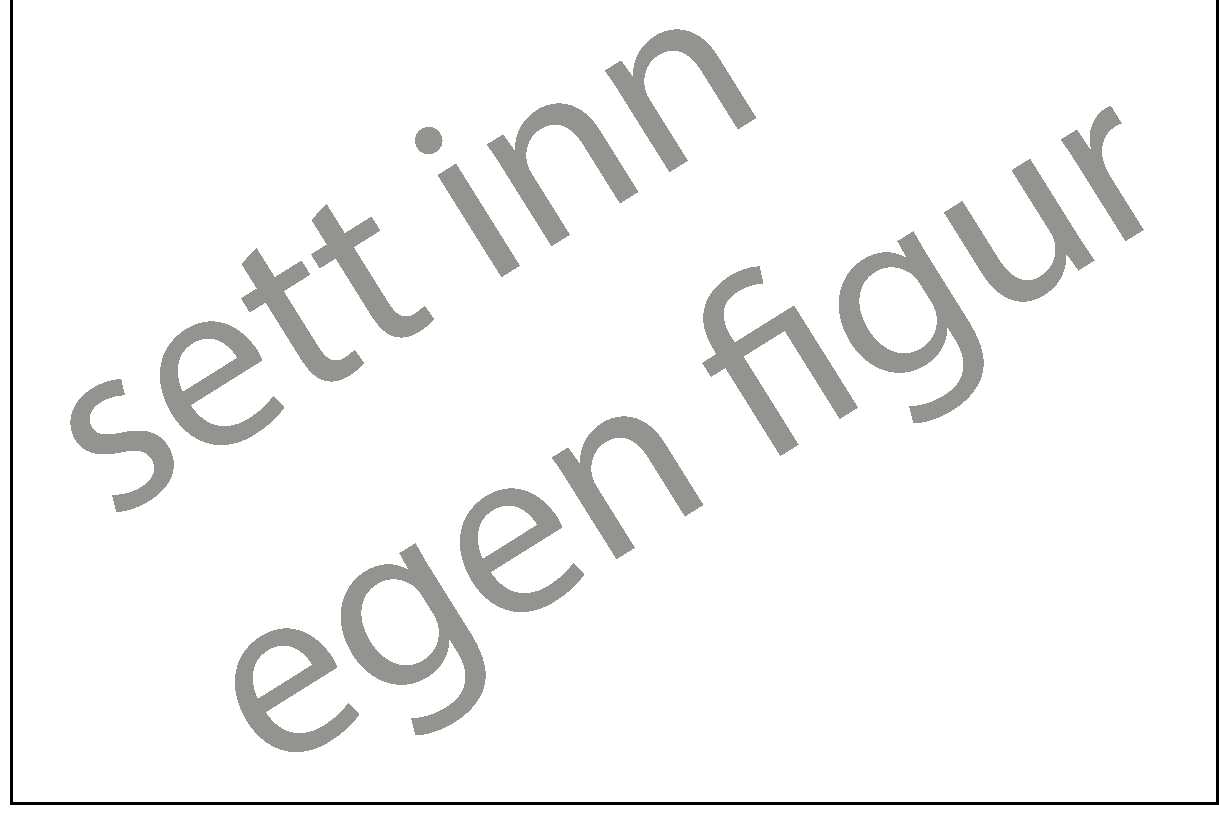
\includegraphics{sett_inn_egen_fig.pdf}}
      \caption{Resultat av blokkskjemaet i modellen. }
      \label{fig:3a}
    \end{figure}

  \item Svaret er gitt i ligning~\eqref{eq:losn1}.
    \begin{equation}
      \label{eq:losn1}
      y = 4
    \end{equation}

  \item Eksempel på bruk av {\tt align} er vist i
    ligning~\eqref{eq:integral}.
    For å bruke kommandoen {\tt \textbackslash uuline} må du bruke pakken
    {\tt ulem} som {\tt \textbackslash usepackage\{ulem\}}.
    \begin{align}
      A   & = \int_{0}^{1} 2{\cdot}\sin(5{\cdot}t) dt \notag \\ 
          & =    -\frac{2}{5}{\cdot}\cos(5{\cdot}t) \Biggl|_{0}^{1}  \notag \\
          &=-\frac{2}{5}{\cdot}\cos(5{\cdot} 1)
            -\Bigl(-\frac{2}{5}\cos(0)\Bigl) \notag\\
          &= \uuline{0.287} \label{eq:integral}
    \end{align}

  \item Du finner også mye \LaTeX-kode i hver av .tex-filene til delxoppgavene.
    
  \end{itemize}
\end{tcolorbox}





\newpage

\section*{Numerisk integrasjon og derivasjon}
\label{side:1}


\begin{enumerate}[a)]

  % ********************************************************
  % oppgave a)
  % ********************************************************
  \runningheader{Introduksjon numerisk integrasjon og derivasjon}{}{Side \thepage\ av \numpages}

\item[] I deloppgaven \ref{oppg:a})-\ref{oppg:e}) skal du jobbe med følgende signal
\begin{equation}
  \label{eq:u}
 \boxed{ u(t) = 2 {\cdot} t^{2} }
\end{equation}
Basert på det diskret signalet $u_{k}$ gjeldende ved
tidspunktene  $t_{k}$ skal 
du numerisk integrere $u_{k}$ og beregne
{\color{blue}\fbox{$y_{k}$}}  
som en tilnæring til operasjonen
\begin{equation}
  y(t)=\int_{0}^{t}u(\tau)d\tau + y(0) \quad \text{gitt } y(0){=}0   \label{eq:y}
\end{equation}
Videre  skal du numerisk derivere  $u_{k}$ for å beregne
{\color{red}\fbox{$v_{k}$}} som en tilnærming til
\begin{equation}
  \label{eq:v}
  v(t) = \frac{d}{dt}u(t)
\end{equation}

Fra matematikken vet du at de analytiske uttrykkene for $y(t)$ og
$v(t)$ er
\begin{equation}
  \label{eq:9}
  {\color{blue}\boxed{y(t) = \frac{2}{3} {\cdot}t^{3}} }
\end{equation}

\begin{equation}
          {\color{red}\boxed{v(t) = 4{\cdot}t}}   \label{eq:9a}
\end{equation}

Disse skal du benytte som ``fasit'' i noen av oppgavene
slik at du visuelt kan sammenligne  med de numeriske beregningene av  
{\color{red}\fbox{$v_{k}$}} og {\color{blue}\fbox{$y_{k}$}}.
Bruken av {\color{red}\fbox{rød}} og {\color{blue}\fbox{blå}} farger
brukes til å skille mellom henholdsvis derivering og integrering.

\newpage

\runningheader{Oppgave a), frivillig}{}{Side \thepage\ av \numpages}

% ********************************************************
% oppgave a) 
% ********************************************************  
\item
  {\bf Numerisk integrasjon og derivasjon i Simulink}
\label{oppg:a}

  
\begin{itemize}
\item Ta utgangspunkt i Simulinkmodellen i skallfilen
  \fbox{\tt oving3\_a\_m\_skallfil.slx}  vist i figur~\ref{fig:1a_dump},
    og implementer ligning~\eqref{eq:u} og de to analytiske løsningene i
    ligning~\eqref{eq:9} og 
    \eqref{eq:9a} i hvert sitt tilhørende subsystem. Bruk
    blokkene \fbox{\tt Clock}, \fbox{\tt Math Function}  hvor du velger \fbox{\tt
      pow} fra rullegardinmenyen,   samt  \fbox{\tt  Product}
    for å lage disse signalene.  {\color{black}Ta med skjermdump av
      de 3 delmodellene i innleveringen.} 
    \begin{figure}[H]
      \centering
      \hspace*{0mm}\scalebox{0.85}{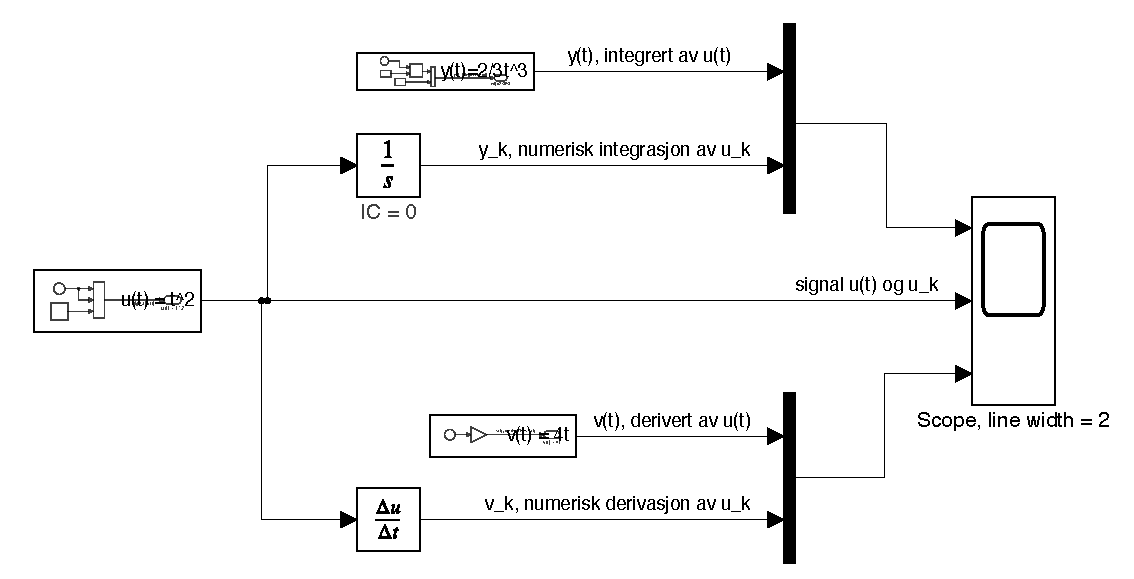
\includegraphics{3a_modell.pdf}}
      \caption{Simulinkmodell hvor ligningene~\eqref{eq:u}, \eqref{eq:9} og 
    \eqref{eq:9a} er implementert i hvert sitt subsystem. }
      \label{fig:1a_dump}
    \end{figure}

    For å sammenligne analytiske og numeriske resultat 
    velger vi å bruke tidspunkt $t{=}2$~sekund. De 
    analytiske verdiene ved dette tidspunktet finner vi fra ligningene~\eqref{eq:9}
    og \eqref{eq:9a} som
    \begin{equation}
      \label{eq:92}
      {\color{blue}{y(2) = \frac{2}{3} {\cdot}2^{3}=5.333}}       
    \end{equation}
    \begin{equation}
      {\color{red}{v(2)  = 4{\cdot}2 = 8}}  \label{eq:9a2}       
    \end{equation}

    For å lese av de  tilsvarende verdiene {\color{blue}\fbox{$y_{k}$}} og
      {\color{red}\fbox{$v_{k}$}} ved $t_{k}{=}2$ sekund i scopet, er
      scopet i skallfilen klargjort med  kurveavlesingsverktøyet
      hentet fra\\ \fbox{\tt Tools -> Measurements -> Cursor
        Measurements}.\\

      Det er  huket av for  \fbox{\tt Snap to data},
      men du må selv velge hvillket signal du skal lese av (i
      skallfilen er  begge avlesningene på $u_{k}$).
      I skallfilen har vi lagt  på markør på kurvene for å fremheve
      beregningstids\-punktene.

      \newpage
\item Spesifiser {\it Eulers forovermetode} ({\tt ode1}) med
  steglengde lik $T_{s}{=}0.4$ sekund, simuler modellen i 3 sekund og
  vis at du får følgende respons
  \begin{figure}[H]
    \centering
    \hspace*{10mm}\scalebox{0.5}{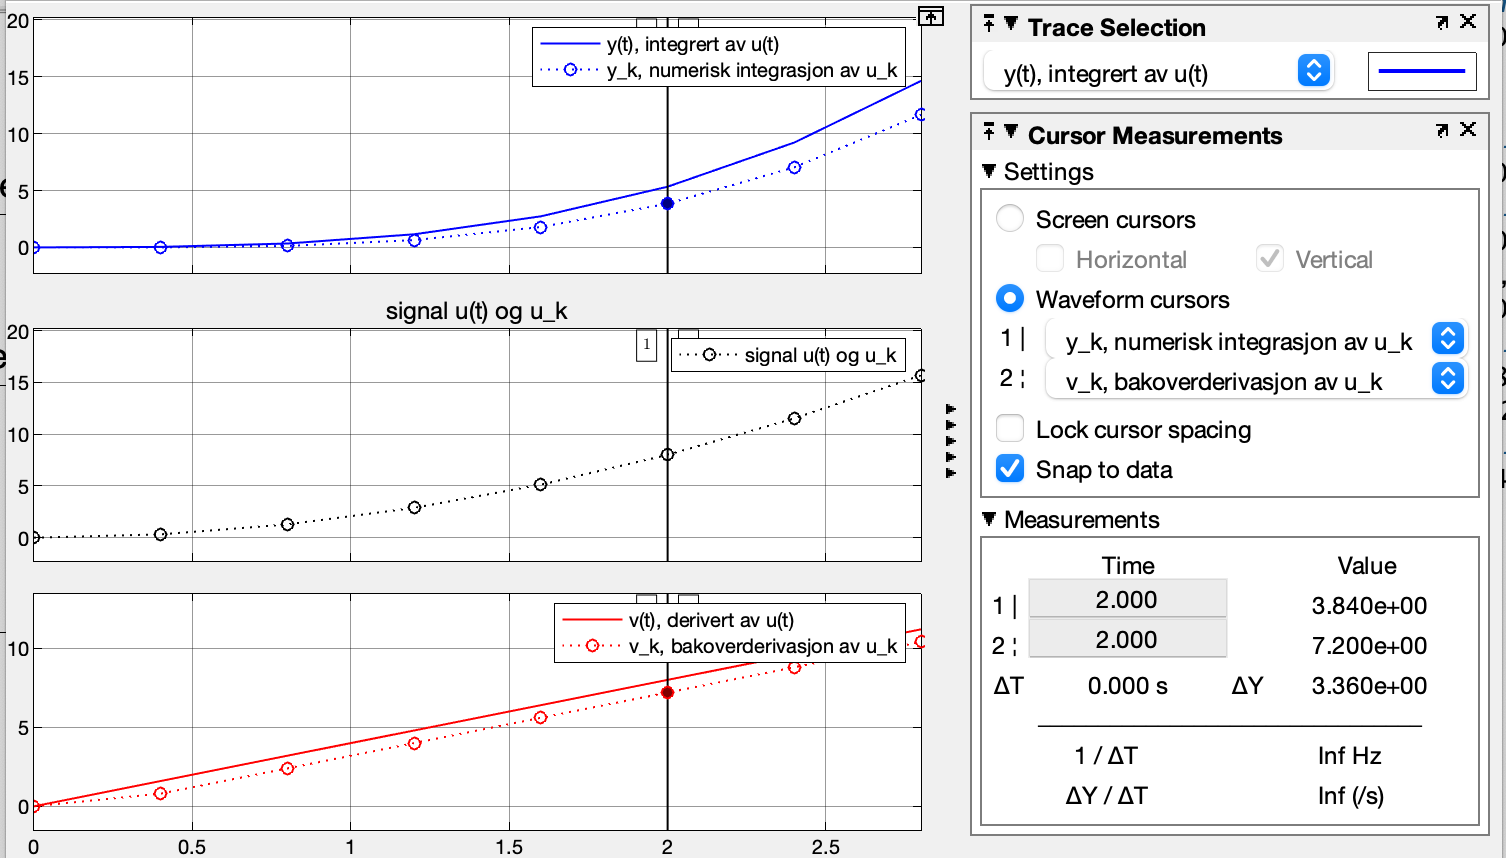
\includegraphics{oppg3a_1.png}}
    \caption{Simuleringsresultat }
    \label{fig:oppg3_1}
  \end{figure}
  
  Ta med din egen respons inkludert avlesingene i innleveringen, og
  vis som over at de avleste verdiene ved $t_{k}{=}2$ sekund er
  \begin{equation}
    {\color{blue}{y_{k}=3.840}}  
  \end{equation}
  \begin{equation}
  {\color{red}{v_{k}=7.2}}   
  \end{equation}
  
      

  \item 
    Spesfiser deretter {\it Eulers bakovermetode} ({\tt ode1be}) med
    samme steglengde og simuler på
    ny. Avles {\color{blue}\fbox{$y_{k}$}} og
    {\color{red}\fbox{$v_{k}$}}  ved samme tidspunkt.
    Ta med din egen respons inkludert avlesingene i innleveringen.

    Gi en forklaring på endringen i den avleste verdien for
    {\color{blue}\fbox{$y_{k}$}}. Gi også en forklaring på hvorfor 
    {\color{red}\fbox{$v_{k}$}} er uendret.


  \item 
    Spesfiser deretter {\it Heuns metode} ({\tt ode2}) som tilsvarer
    {\it trapesmetoden},  og simuler på
    ny. Avles igjen {\color{blue}\fbox{$y_{k}$}} og
      {\color{red}\fbox{$v_{k}$}}  ved samme tidspunkt.
    Ta med din egen respons inkludert avlesingene i innleveringen.

    Gi også her en forklaring på endringen i den avleste verdien for
    {\color{blue}\fbox{$y_{k}$}}. 

\end{itemize}
  

  \begin{tcolorbox}[breakable, enhanced]
    \subsection*{Svar}
    
    
  \end{tcolorbox}




  % ********************************************************
  % oppgave b)
  % ********************************************************
  \newpage
  \runningheader{Oppgave b)}{}{Side \thepage\ av \numpages}
% ********************************************************
% oppgave b) 
% ********************************************************  
\item
{\bf Numerisk integrasjon og derivasjon i Matlab}
\label{oppg:b}

I denne oppgaven skal du ta
utgangspunkt   i skallfilen \fbox{\tt oving3\_skallfil.m} for å  
lage kode for numerisk
integrasjon av
$u(t)$ fra ligning~\eqref{eq:u} ved å bruke både {\it Eulers  forovermetode},
  {\it  Eulers  bakovermetode} og {\it  trapes\-metoden}, henholdsvis gitt som:
  \begin{alignat}{3}
    &y_{k} && =  y_{k-1} +
              T_s {\cdot} u_{k-1}, 
    &&~~ \forall ~  k{=}2,\ldots,n \quad \text{gitt } y_{1} \label{eq:ef}\\
    &y_{k} && =  y_{k-1} +
              T_s {\cdot} u_{k}, 
    &&~~\forall ~  k{=}2,\ldots,n\quad \text{gitt } y_{1} \label{eq:eb}\\
    &y_{k} && =  y_{k-1} +
              T_s {\cdot} \frac{1}{2}{\cdot} \bigl(u_{k-1} + u_{k} \bigr),
    &&~~\forall ~  k{=}2,\ldots,n \quad \text{gitt } y_{1} \label{eq:tr}
  \end{alignat}
  
  
  Du skal også utføre kodebasert numerisk derivasjon   av
$u(t)$ ved å bruke både {\it bakoverderivasjon}, 
  {\it  foroverderivasjon}, 
  og {\it  senter\-derivasjon}, henholdsvis  gitt som 
  \begin{alignat}{3}
    & v_{k} && =\frac{u_{k}-u_{k-1}}{T_s}, &&\quad  \forall ~
            k{=}2,\ldots,n \quad \text{gitt } v_{1}=0 \label{eq:bak}\\
    & v_{k-1} && =\frac{u_{k}-u_{k-1}}{T_s},&&\quad\forall ~ k{=}2,\ldots,n\\
    & v_{k-1} && =\frac{u_{k}-u_{k-2}}{2{\cdot}T_s}, &&\quad\forall ~
              k{=}3,\ldots,n \quad \text{gitt } v_{1}=0
  \end{alignat}
   
  \begin{itemize}
  \item Ferdigstill den uferdige koden for denne deloppgaven, og
    vis at du får følgende resultat (ta med din egen figur
    i innleveringen).
    \begin{figure}[H]
      \centering
      \hspace*{10mm}\scalebox{0.45}{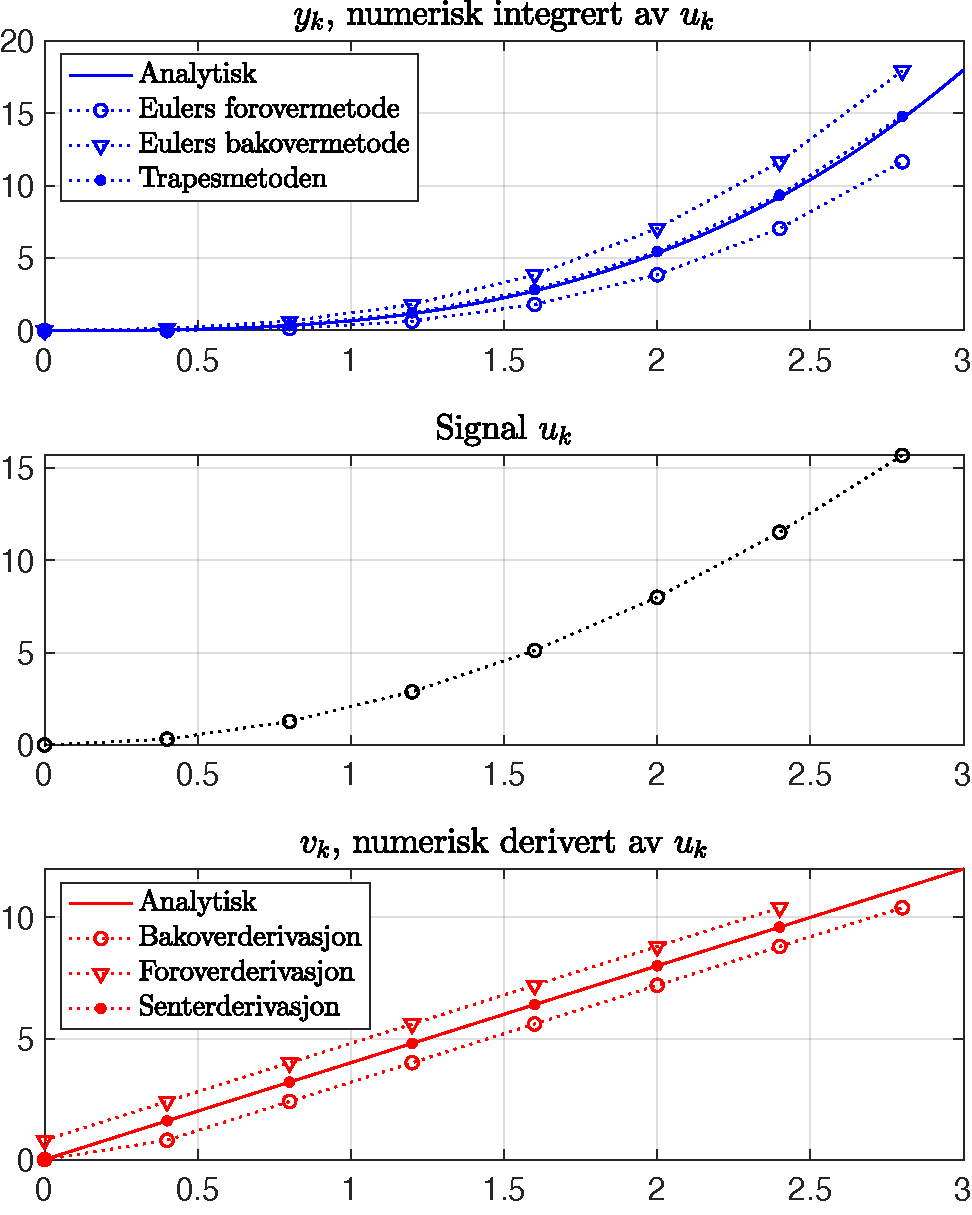
\includegraphics{fig3b_1.pdf}}
      \caption{Simuleringsresultat }
      \label{fig:fig3b_1}
    \end{figure}


  Når du skal plotte forover- og senterderivasjon,
  så må du passe på at dimensjonene til tidsvektoren og henholdsvis
  {\tt  v\_forover(k)} og  {\tt v\_senter(k)} er like lange. 
  
\item
  Avles verdiene av  {\tt y\_EulerF(k)},  {\tt y\_EulerB(k)} og
  {\tt y\_Trapes(k)} ved tidspunkt $t_{k}{=}2$~sekund som i
  deloppgave~\ref{oppg:a}), og vis at de er identiske med
  {\color{blue}\fbox{$y_{k}$}}-verdiene du fant der.

\item
  Avles verdien av  {\tt v\_bakover(k)} 
  ved tidspunkt $t_{k}{=}2$~sekund som i
  deloppgave~\ref{oppg:a}), og vis at den er identiske med
 alle tre {\color{red}\fbox{$v_{k}$}}-verdiene du fant der. 
  \end{itemize}

  

  \begin{tcolorbox}[breakable, enhanced]
    \subsection*{Svar}
    
    
  \end{tcolorbox}




  % ********************************************************
  % oppgave c)
  % ********************************************************
  \newpage
  \runningheader{Oppgave c), frivillig}{}{Side \thepage\ av \numpages}
% ********************************************************
% oppgave c) 
% ********************************************************  
\item
{\bf Numerisk integrasjon og derivasjon for hånd}
\label{oppg:c}

For å få litt eksamenstrening, skal du gjøre numerisk integrasjon og
  derivasjon for hånd basert på et begrenset datasett. 
  Vi tar utgangspunkt i de fem første tidspunktene i $t_{k}$ gitt som
  \begin{equation}
    \label{eq:2}
  t_{k}=[0,~0.4,~0.8,~1.2,~1.6,~2]    
  \end{equation}
De tilhørende  verdiene for  $u_{k}$ er 
  \begin{align}
    \label{eq:1g}
    u_{k} &= 2{\cdot} t_{k}^{2} \\
    & = [0,~    0.32,~    1.28,~    2.88,~    5.12, ~8] 
  \end{align}

  \begin{itemize}
  \item 
  Bruk {\it Eulers forovermetode} 
  til manuelt å beregne det numeriske integralet av
  $u_{k}$, som betyr å finne 
  \begin{equation}
    \label{eq:1}
    y_{k}  =  y_{k-1} +  T_s {\cdot} u_{k-1}, 
    \quad \forall~ k=2,\ldots ,6, \quad \text{gitt } y_{1}=0
  \end{equation}
  
  \item 
  Bruk {\it bakoverderivasjon} til
  manuelt å beregne den numeriske deriverte av $u_{k}$, som betyr å finne
  \begin{equation}
     v_{k} =\frac{u_{k}-u_{k-1}}{T_s}, \quad  \forall ~
            k{=}2,\ldots,6 \quad \text{gitt } v_{1}=0 \\
  \end{equation}
  \end{itemize}
  

  \begin{tcolorbox}[breakable, enhanced]
    \subsection*{Svar}
    
    
  \end{tcolorbox}


  
  % ********************************************************
  % oppgave d)
  % ********************************************************
  \newpage
  \runningheader{Oppgave d)}{}{Side \thepage\ av \numpages}
% ********************************************************
% oppgave d) 
% ********************************************************  
\item
{\bf Numerisk integrasjon som Matlab-funksjon}
\label{oppg:d}

I denne oppgaven skal du lage en egen funksjon av
Eulers forovermetode for numerisk integrasjon.
Du kan også velge å gjøre en frivillig ekstraoppgave hvor du
implementerer alle tre metodene for numerisk integrasjon, og spesifiserer i
funksjonskallet  hvilken metode du vil bruke.
For introduksjon til
funksjoner i Matlab, skriv {\color{red}\fbox{\tt doc function}} i {\tt Command Window}. 



  \begin{itemize}
  \item  Koden i skallfilen kaller på
    funksjonen {\tt EulerForover} som vist under
\begin{lstlisting}[caption={Kodeutdrag som kaller på funksjonen {\tt EulerForover}.},
language= Matlab, label=kode:funksjon_EF,
numbers=none]
y(1) = 0;  % initialverdi
for ..
    y(k) = EulerForover(.. , .., ..);
end
\end{lstlisting}

Med utgangspunkt i Eulers forovermetode gitt som
\begin{equation}
  \label{eq:1aa}
  y_{k}  =  y_{k-1} +  T_s {\cdot} u_{k-1}
\end{equation}
fullfør koden i skallfilen til funksjonen  
\fbox{\tt  EulerForover.m}, gjengitt under.

\begin{lstlisting}[caption={Funksjonen/filen {\tt EulerForover.m}.},
language= Matlab, label=kode:funksjon_EF2,
numbers=none]
function IntValueNew = EulerForover(IntValueOld, Timestep, FunctionValue)
% fyll inn
end
\end{lstlisting}

    Som du ser benytter funksjonen variabelnavn som er matematisk  
    beskrivende, samtidig som at den ikke skal benytte indeks
    {\tt k}.

    \item Kjør koden  og vis at {\tt y(k)} gir samme resultat som 
    {\tt  y\_EulerF(k)} i oppgave~\ref{oppg:b}).
\end{itemize}


    

\newpage
\subsubsection*{Generell funksjon for numerisk integrasjon (frivillig)}

For å ha en mer fleksibel integrasjonsrutine skal vi lage en ny
funksjon hvor vi inkluderer et argument som sier noe om hvilken
metode som skal brukes.
Et utgangspunkt for dette er funksjonen {\tt Integrasjon} vist i
kode~\ref{kode:funksjon_num_int}, og  
denne finner du igjen i skallfilen \fbox{\tt Integrasjon.m}.
  

\begin{lstlisting}[caption={Den utvidede funksjonen/filen {\tt Integrasjon.m}.},
language= Matlab, 
label=kode:funksjon_num_int,
 numbers=none]
function IntValueNew = Integrasjon(IntValueOld, Timestep, FunctionValues, options)

arguments
    IntValueOld (1,1) double             % spesifiserer som skalar, 1x1
    Timestep (1,1) double                % spesifiserer som skalar, 1x1
    FunctionValues (1,2) double          % spesifiserer som vektor, 1x2
    options.metode (1,:) char = 'Trapes' % metodevalg, default er Trapes
end
    
if strcmp(options.metode,'EulerForover')
    % fyll inn
elseif strcmp(options.metode,'EulerBakover')
    % fyll inn
elseif strcmp(options.metode,'Trapes')
    % fyll inn
else
    errordlg('Feil metode spesifisert')
    return
end
end
\end{lstlisting}

For å kalle på denne 
funksjonen benyttes syntaksen vist i
kode~\ref{kode:funksjon_num_int_kall} hvor du ser at de to siste elementene
{\tt  u(k-1:k)} sendes inn, uansett  metodevalg. Du må derfor passe å plukke ut riktig
element for hver metode i funksjonen.  

\begin{lstlisting}[caption={Alternativ bruk av funksjonen {\tt Integrasjon}.},
language= Matlab,  label=kode:funksjon_num_int_kall,
linewidth=13.5cm, numbers=none]
y(k) = Integrasjon(y(k-1), T_s, u(k-1:k), metode='EulerForover');
y(k) = Integrasjon(y(k-1), T_s, u(k-1:k), metode='EulerBakover');
y(k) = Integrasjon(y(k-1), T_s, u(k-1:k), metode='Trapes');
y(k) = Integrasjon(y(k-1), T_s, u(k-1:k));   % default: Trapes
\end{lstlisting}

 Vis at ved å kjøre koden så får du resultatet vist i figur~\ref{fig:3d3}. 

\begin{itemize}
  \item Lek litt med å øke og/eller redusere på steglengden \fbox{\tt
      T\_s} i linje 5, og studer effekten på integralene.   
\end{itemize}



    \begin{figure}[H]
      \centering
      \hspace*{0mm}\scalebox{0.6}{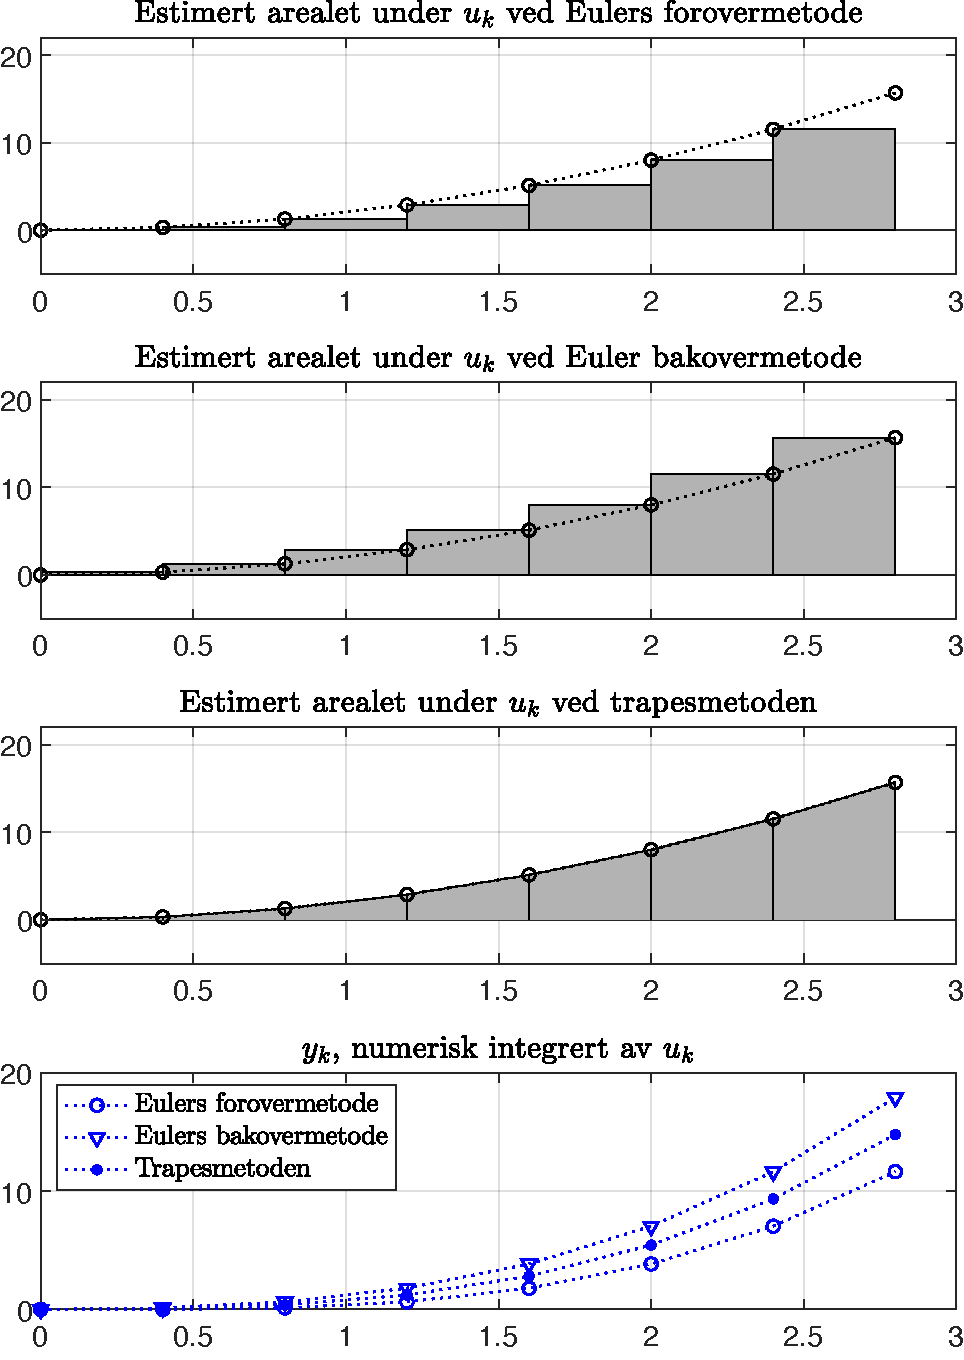
\includegraphics{fig3d_2.pdf}}
      \caption{Presentasjon av arealet under  kurven $u_{k}$ for de
        tre integrasjonsmetodene ved å bruke henholdsvis 
        {\color{red}\fbox{\tt bar}} og {\color{red}\fbox{\tt area}}-kommandoene.}
      \label{fig:3d3}
    \end{figure}

  

  \begin{tcolorbox}[breakable, enhanced]
    \subsection*{Svar}
    
    
  \end{tcolorbox}


  
  

  % ********************************************************
  % oppgave e)
  % ********************************************************
  \newpage
  \runningheader{Oppgave e)}{}{Side \thepage\ av \numpages}
% ********************************************************
% oppgave e) 
% ********************************************************  
\item
  {\bf Numerisk derivasjon som Matlab-funksjon}
\label{oppg:e}
  
  I denne oppgaven skal du lage en egen funksjon av
  bakoverderivasjon. På samme måte som i deloppgave~\ref{oppg:d}) kan
  du velge å  gjøre den frivillige ekstraoppgaven hvor du implementerer alle tre
  metodene og spesifiserer i funksjonskallet hvilken metode du vil
  bruke.

  
  \begin{itemize}
  \item  Koden i skallfilen kaller på
    funksjonen {\tt BakoverDerivasjon} som vist under

\begin{lstlisting}[caption={Kodeutdrag som kaller på funksjonen {\tt BakoverDerivasjon}.},
language= Matlab,  label=kode:bakover2, numbers=none] 
v(1) = 0;   %initialverdi
for ..
    v(k) = BakoverDerivasjon( .., ..);
end
\end{lstlisting}

Med utgangspunkt i bakoverderivasjon gitt som
    \begin{equation}
      \label{eq:1ab}
      v_{k} =\frac{u_{k}-u_{k-1}}{T_s}
    \end{equation}
fullfør koden i skallfilen til funksjonen  
\fbox{\tt  BakoverDerivasjon.m}, gjengitt under.

\begin{lstlisting}[caption={Funksjonen/filen {\tt BakoverDerivasjon.m}.},
language= Matlab,  label=kode:bakover, numbers=none] 
function Sekant = BakoverDerivasjon(FunctionValues, Timestep)
% fyll inn
end
\end{lstlisting}

    Som du ser benytter funksjonen variabelnavn som er matematisk  
    beskrivende, og den skal formuleres uten bruk av indeks {\tt k}. 
\item Kjør koden  og vis at {\tt v(k)} gir samme resultat som 
    {\tt  v\_bakover(k)} i oppgave~\ref{oppg:b}).
  
\end{itemize}

\newpage
\subsubsection*{Generell funksjon for numerisk derivasjon (frivillig)}

For å ha en mer fleksibel derivasjonsrutine skal vi lage en ny
funksjon hvor vi inkluderer et argument som sier noe hvilken
metode som skal brukes.
Et utgangspunkt for dette er funksjonen
{\tt  Derivasjon} vist i kode~\ref{kode:funksjon_num_der}, og denne
finner du igjen i skallfilen \fbox{\tt Derivasjon.m}.

\begin{lstlisting}[caption={Utvidet funksjon for numerisk derivasjon.},
language= Matlab, 
numbers=none,  label=kode:funksjon_num_der]
function Sekant = Derivasjon(FunctionValues, Timestep, options)
arguments
    FunctionValues (1,3) double          % spesifiserer som vektor, 1x3
    Timestep (1,1) double                % spesifiserer som skalar, 1x1
    options.metode (1,:) char = 'Bakover' % metodevalg, default er Bakover
end
    
if strcmp(options.metode,'Forover')
     % fyll inn

elseif strcmp(options.metode,'Bakover')
     % fyll inn

elseif strcmp(options.metode,'Senter')
     % fyll inn

else
    errordlg('Feil metode spesifisert')
    return
end

end
\end{lstlisting}

For å kalle denne funksjonen benyttes syntaksen vist i
kode~\ref{kode:funksjon_num_der_kall} hvor du
ser at de tre siste elementene {\tt  u(k-2:k)}
sendes inn, uansett  metodevalg. Du må derfor passe å plukke ut riktig
element for hver metode i funksjonen.



\begin{lstlisting}[caption={Alternativ bruk av funksjonen {\tt Derivasjon}.},
language= Matlab,  label=kode:funksjon_num_der_kall, numbers=none]
v(k)   = Derivasjon(u(k-2:k), T_s, metode='Bakover');
v(k-1) = Derivasjon(u(k-2:k), T_s, metode='Forover');
v(k-1) = Derivasjon(u(k-2:k), T_s, metode='Senter');
\end{lstlisting}

For å sende inn tre verdier av {\tt u} så kan ikke funksjonen
kalles på før $k{=}3$. Det betyr også at noe må gjøres med
initialverdiene, og dette er vist i skallfilen.

Vis at ved å kjøre koden så får du resultatet vist i figur~\ref{fig:3e_o}. 

    \begin{figure}[H]
      \centering
      \hspace*{0mm}\scalebox{0.5}{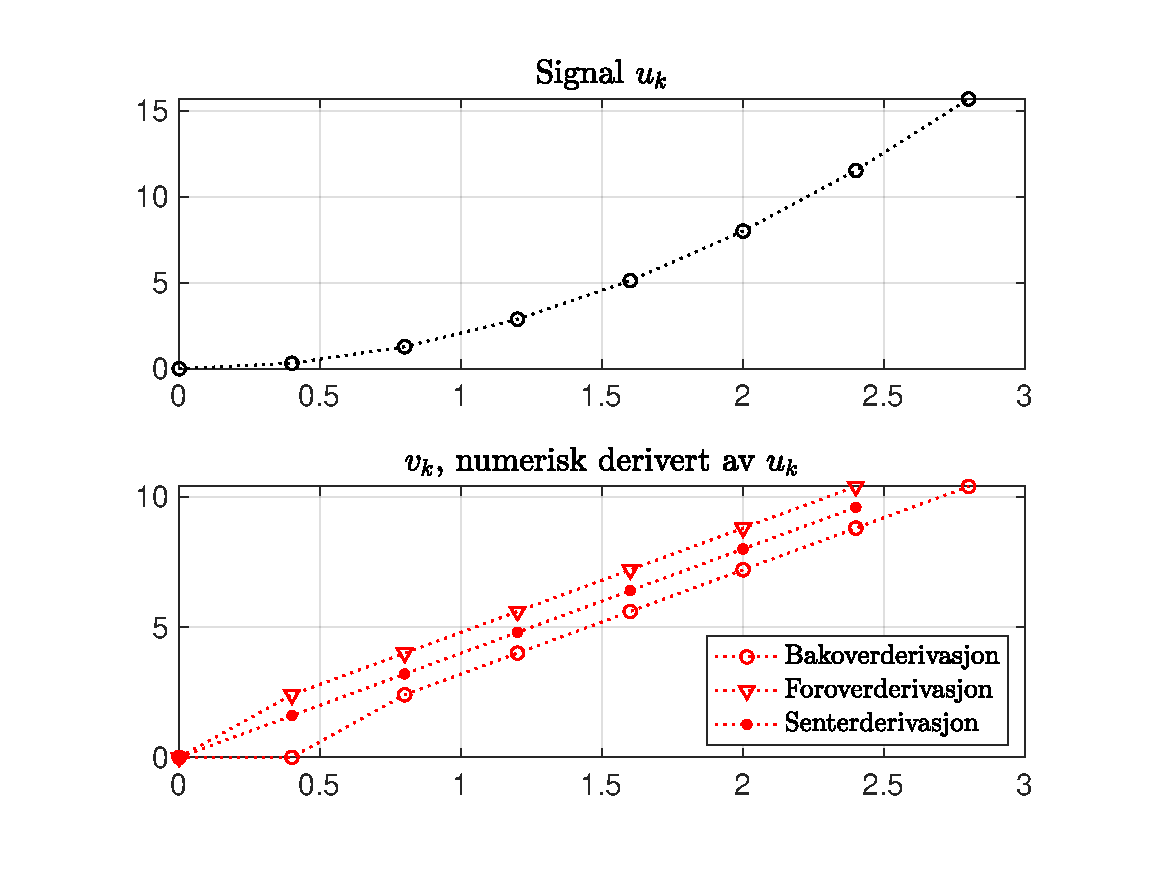
\includegraphics{fig3e_1.pdf}}
      \caption{Resultat av numerisk derivasjon ved bruk av funksjonen
        {\tt Derivasjon}. }
      \label{fig:3e_o}
    \end{figure}
  

  \begin{tcolorbox}[breakable, enhanced]
    \subsection*{Svar}
    
    
  \end{tcolorbox}



3 \newpage
  
  \section*{Viktige egenskaper ved numerisk integrasjon og derivasjon}

  % ********************************************************
  % oppgave f)
  % ********************************************************
  \runningheader{Oppgave f)}{}{Side \thepage\ av \numpages}

\item[] I de neste to deloppgavene \ref{oppg:f})-\ref{oppg:g}) skal du
  jobbe med følgende enkle signal
\begin{equation}
  \label{eq:u2}
 \boxed{ u(t) = 1 }
\end{equation}
Hensikten med å bruke et såpass enkelt signal er å demonstrere 
noen viktige egenskaper ved numerisk integrasjon og derivasjon.


% ********************************************************
% oppgave f) 
% ********************************************************  
\item
{\bf Numerisk integrasjon av et signal som er forsterket}
\label{oppg:f}

I denne oppgaven skal du beregne følgende integral 
\begin{equation}
  \label{eq:4aa}
  y(t) = K_{i}  \int_{0}^{t}  u(t)dt
\end{equation}
ved å bruke  funksjonen {\tt EulerForover} fra deloppgave~\ref{oppg:d}). 
Parameteren $K_{i}$ er en forsterkningsfaktor som kan være et vilkårlig tall,
positivt eller negativt. 
I koden nedenfor er $K_{i}{=}0.4$, og det er implementert to forskjellig varianter av
numerisk integrasjon. Den ene varianten er riktig, den
andre er feil, og målet med oppgaven er at du skal finne ut hvilken
som er riktig, og forklare hvorfor det er slik.
\vspace*{-5mm}
\begin{lstlisting}[caption={Kode for oppgaven.},
language= Matlab, label=kode:1f, numbers=none] 
% initialverdi
y1(1) = 0;
y2(1) = 0;

Ki = 0.4;
for k = ..
    y1(k) =    EulerForover(y1(k-1), T_s, Ki*u(k-1));
    y2(k) = Ki*EulerForover(y2(k-1), T_s,    u(k-1));
end
\end{lstlisting}
\begin{itemize}
\item Pass på at \fbox{\tt Ki = 0.4;} og kjør koden. Kan du allerede
  nå ut fra kurvene finne ut om det er {\tt y\_1} eller {\tt y\_2} som er riktig?

\item Endre parameteren $K_{i}$ til \fbox{\tt Ki = 1.4;} og kjør
  koden på ny. Blir du noe klokere av det? 

\item For å bli sikker på svaret er det smart å legge inn følgende kode
  i linjen etter at {\tt u} blir definert.  

\begin{lstlisting}[numbers=none]
u(5:end) = 0;  % setter siste del av u som 0
\end{lstlisting}

Du kan nå endre $K_{i}$ mellom \fbox{\tt Ki = 0.4;} og \fbox{\tt
  Ki = 1.4;}, og du vil forhåpetligvis oppdage hvilken som er den
riktige.

\item Hva er den egentlige grunnen til at den som er feil, er feil.
  
\end{itemize}
  

  \begin{tcolorbox}[breakable, enhanced]
    \subsection*{Svar}
    
    
  \end{tcolorbox}




  % ********************************************************
  % oppgave g)
  % ********************************************************
  \newpage
  \runningheader{Oppgave g), frivillig}{}{Side \thepage\ av \numpages}
% ********************************************************
% oppgave g) 
% ********************************************************  
\item
{\bf Effekten av støy ved numerisk derivasjon}
\label{oppg:g}

For å gjøre denne oppgaven må du gjort 
de frivillige oppgavene i~\ref{oppg:d}) og \ref{oppg:e}). 

Hensikten med oppgaven er å studere effekten av støy ved numerisk
integrasjon og derivasjon. Vi tar utgangspunkt i signalet fra
ligning~\eqref{eq:u2} hvor vi lager et signal uten støy som vi kaller
\fbox{\tt u1}, og et signal med støy som vi kaller \fbox{\tt u2}.

Vi benytter deretter Eulers forovermetode på begge signalene for å
beregne henholdsvis \fbox{\tt y1} og \fbox{\tt y2}.

I tillegg benytter vi bakoverderivasjon på begge signalene for å
beregne henholdsvis \fbox{\tt v1} og \fbox{\tt v2}.
For å studere effekten av metodevalg for derivasjon,
benytter vi senterderivasjon på signalet med støy og beregner \fbox{\tt v3}. 

\begin{itemize}
\item 
  Pass på at \fbox{\tt T\_s = 0.4} og kjør koden.
  Endre tidsskrittet i steg fra  \fbox{\tt T\_s = 0.4} til
  \fbox{\tt T\_s =  0.05}.
 Vi at du får et resultatet som ligner på figur~\ref{fig:fig1g_1}.
  Ta med figuren din i innleveringen.
 \begin{figure}[H]
      \centering
      \hspace*{0mm}\scalebox{0.43}{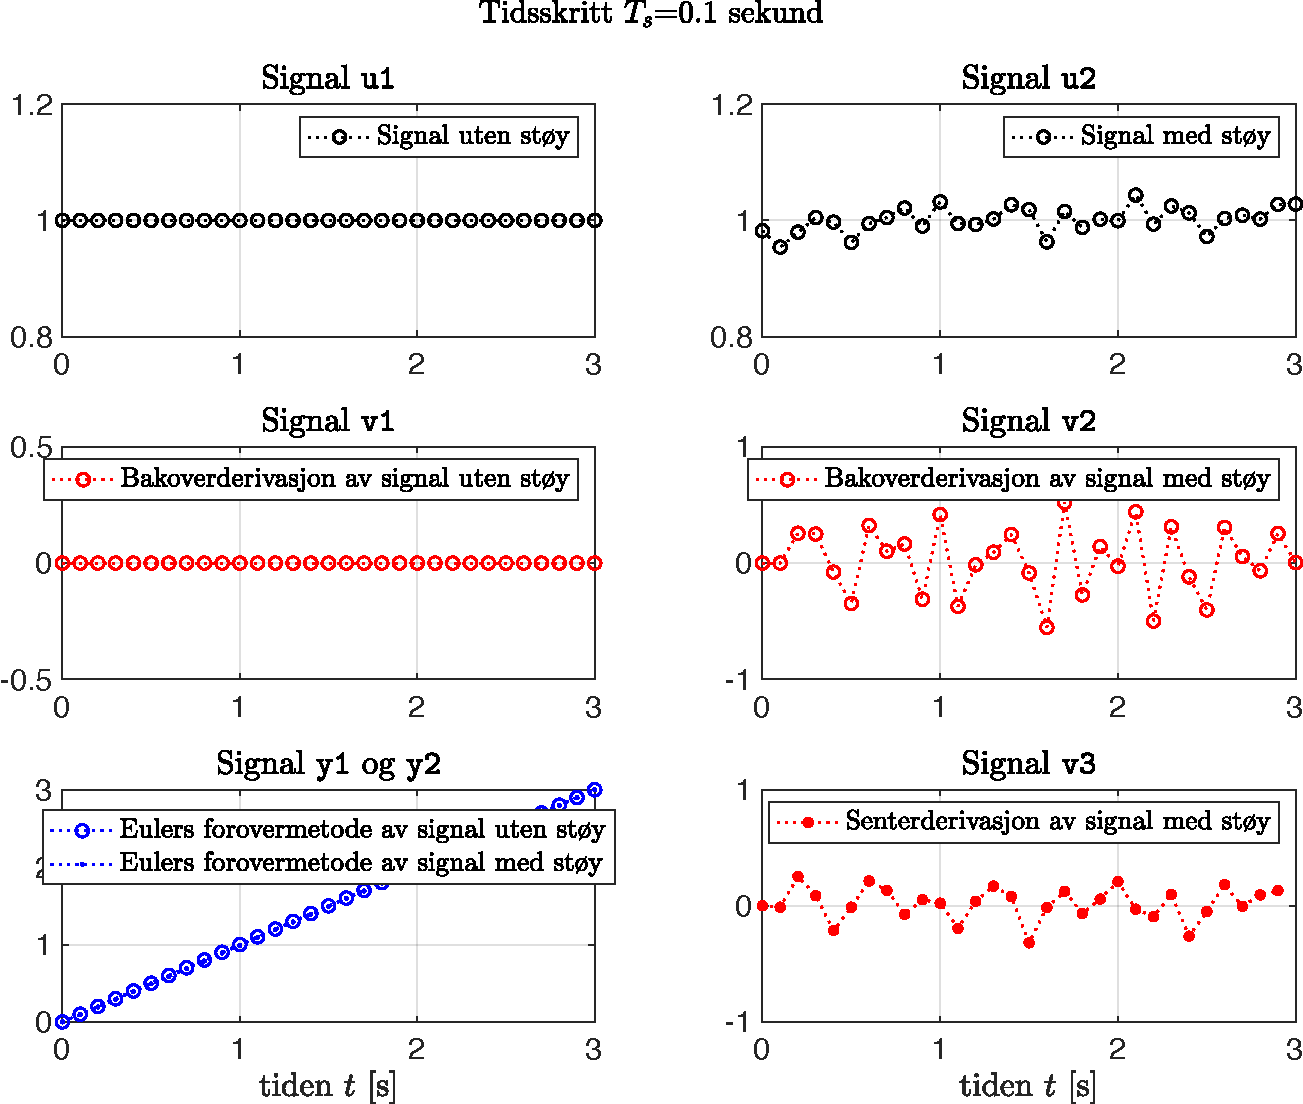
\includegraphics{fig3g_1.pdf}}
      \caption{Resultat som viser hvordan støy påvirker numerisk
        integrasjon og derivasjon.}
      \label{fig:fig1g_1}
    \end{figure}


\item  Hva skjer med signalene
  {\tt v2} og {\tt v3} etterhvert som tidsskrittet synker?
  Hva er forklaringen på at utslaget i
  disse to blir større og større?


\item Forklar hvorfor støy ikke påvirker numerisk
  integrasjon i særlig grad. 

\item Hva er grunnen til at senterderivasjon gir bedre resultat
  sammenlignet med bakoverderivasjon?
 
   
\end{itemize}

  

  \begin{tcolorbox}[breakable, enhanced]
    \subsection*{Svar}
    
    
  \end{tcolorbox}



  

  \newpage

  \label{side:2}
  \section*{Effekten av samplingsfrekvensen $f_{s}$ ved måling}

  % ********************************************************
  % oppgave h)
  % ********************************************************
  \runningheader{Oppgave h)}{}{Side \thepage\ av \numpages}
% ********************************************************
% oppgave h) 
% ******************************************************** 
\item
  {\bf Fenomenet nedfolding}

\label{oppg:h}

  I denne oppgaven tar vi utgangspunkt i hvordan sampling blir utført
  som vist i kapittel 7.2 i kompendiet. 
  Hensikten med oppgaven er å demonstrere hvilken betydningen
  samplingsfrekvensen  $f_{s}$~[Hz] har ved sampling av signaler som
  består av forskjellige frekvenser $f$~[Hz].  Vi skal derfor bruke
  følgende 5 cosinussignal
\begin{align}
  x_{1}(t) & =   \cos(2\pi f_{1} {\cdot}t)  \label{eq:U1} \\
  x_{2}(t) & =   \cos(2 \pi f_{2} {\cdot}t)  \label{eq:U2} \\
  x_{3}(t) & =   \cos(2\pi f_{3} {\cdot}t)  \label{eq:U3}\\
  x_{4}(t) & =   \cos(2\pi f_{4} {\cdot}t)  \label{eq:U4}\\
  x_{5}(t) & =   \cos(2\pi f_{5} {\cdot}t)  \label{eq:U5}
\end{align}
  hvor vi benytter følgende frekvenser 
\begin{equation}
  f_{1} = 0.1,  ~ f_{2}= 0.3, ~ f_{3}= 0.5, ~ f_{4}= 0.9 ~\text{og}~f_{5}= 1.3
  ~\text{Hz} \notag
\end{equation}
Som du ser i skallfilen lager vi først 
den ``kontinuerlige'' tidsvektoren \fbox{\tt tid}  ved å benytte et
veldig kort tidsskritt \fbox{\tt delta\_t = 0.001}.

Deretter lages  vektoren \fbox{\tt t} med samplingstidspunkt som
representerer de tidspunktene hvor målingene blir tatt. Basert på
tidsvektorene {\tt tid} og {\tt t} lages det deretter  
en {\it analog} og en {\it diskret} versjon av alle fem signalene
\fbox{\tt x\_1} til \fbox{\tt x\_5}. Til slutt summeres alle de analoge signalene til
signalet \fbox{\tt x\_a} og alle de diskret signalene til signalet
\fbox{\tt x\_d}. På denne måten kan du kan se effekten av
samplingsfrekvensen \fbox{\tt f\_s} på et sammensatt 
og mer reelt signal (ikke bare et rent cosinussignal).
%{\color{red}Svar på følgende spørsmål:}
\begin{itemize}
\item 
 Hvor stor er samplingsperioden $T_{s}$ for den valgte  
  samplingsfrekvensen $f_{s}{=}0.6$~Hz?
\item 
 Hvor mange elementer er det i signalet \fbox{\tt x\_a} og
 i signalet \fbox{\tt x\_d}?
\item 
 Forklar hva figuren viser? 
\item 
  Hvilke signal ser det ut som vi sampler i \fbox{\tt subplot(7,1,2)} til \fbox{\tt subplot(7,1,5)}?
  Avles periodetidene $T_{p}$ fra de blå stiplede kurvene og beregn
  de tilsynelatende frekvensene for de diskret signalene.
  Sammenlign med frekvensene for de 
  analoge signalene $x_{2}(t)$ til $x_{5}(t)$. 
\item 
 Hva skjer dersom du spesifserer samplingsfrekvensen som
 $f_{s}{=}1$~Hz? 

\item 
  Hva skjer dersom du spesifserer samplingsfrekvensen som
  $f_{s}{=}1.8$~Hz? 

\item 
   Hva skjer dersom du spesifserer samplingsfrekvensen som
   $f_{s}{=}2.6$~Hz? 

\item  Forklar hva som skjer når samplingsfrekvensen øker.



\end{itemize}
  

  \begin{tcolorbox}[breakable, enhanced]
    \subsection*{Svar}
    
    
  \end{tcolorbox}





  
  \newpage

  \section*{Filtrering}
  \label{side:3}
  % ********************************************************
  % oppgave i)
  % ********************************************************
  \runningheader{Oppgave i)}{}{Side \thepage\ av \numpages}
% ********************************************************
% oppgave i) 
% ******************************************************** 
\item
{\bf FIR-filter}
\label{oppg:i}

I Lego-prosjektet skal du jobbe med 
  FIR-filter (midlingsfilter) gitt som 
\begin{equation}
  \label{eq:MA2}
  y_{k} = \frac{1}{M}\sum_{n=0}^{M-1} x_{k-n}
\end{equation}
hvor $M$ er antall målinger av $x$ som skal være med i midlingen.
I denne oppgaven skal du først implementere kode for filteret i
ligning~\eqref{eq:MA2} og deretter skal du lage en egen
funksjon for FIR-filteret i skallfilen \fbox{\tt FIR\_filter.m}. 

Ta utgangspunkt i skallfilen
hvor du ser at den diskret tidsvektoren
\fbox{\tt t} er basert på en antatt samplingsfrekvens på
  \begin{equation}
    \label{eq:15}
      f_{s} = 10~\text{Hz}
  \end{equation}
  som gir et tidsskritt på
  \begin{equation}
    \label{eq:14}
T_{s} = \frac{1}{f_{s}} = 0.1~\text{sekund}     
  \end{equation}
Med en slutt-tid på 10 sekund  betyr det at vi har 100 målinger
tilgjengelig, og målesignalet \fbox{\tt x} er som du ser bare støy. 
Gjør følgende oppgaver:
\begin{itemize}
\item  Implementer kode for
  FIR-filteret i ligning~\eqref{eq:MA2} i {\it for}-løkken. Vær nøye med
  indeksene.
  
  Der hvor det står {\color{darkgreen}\fbox{\tt \% juster på M her}} så gjelder dette
  for situasjonen hvor $k{<}M$ hvor det ikke er nok
  målinger til å bruke {\tt M = 10}. En måte å løse det på er å utsette
  filtreringen til $k{>}M$, men en bedre løsning er justere på $M$
  slik at filtreringen kan starte med en gang.
  Hint: Hva skulle du ønske at
  $M$ var i starten av filtreringen, og så lenge $k{<}M$?

  Vær
  klar over at siden du gjør justeringer på $M$ inne i {\it for}-løkka
  når $k < M$, så må koden \fbox{\tt M = 10;} stå inne i den samme
  løkka. Setter du koden {\tt M = 10;} foran {\it for}-løkka så vil
  ikke verdien av $M$ bli resatt for hver runde i løkka. Test det
  gjerne ut.

\newpage
  Ferdigstill og kjør koden og vis at du får  resultatet vist i figur~\ref{fig:3i}.
    \begin{figure}[H]
      \centering
      \hspace*{0mm}\scalebox{0.45}{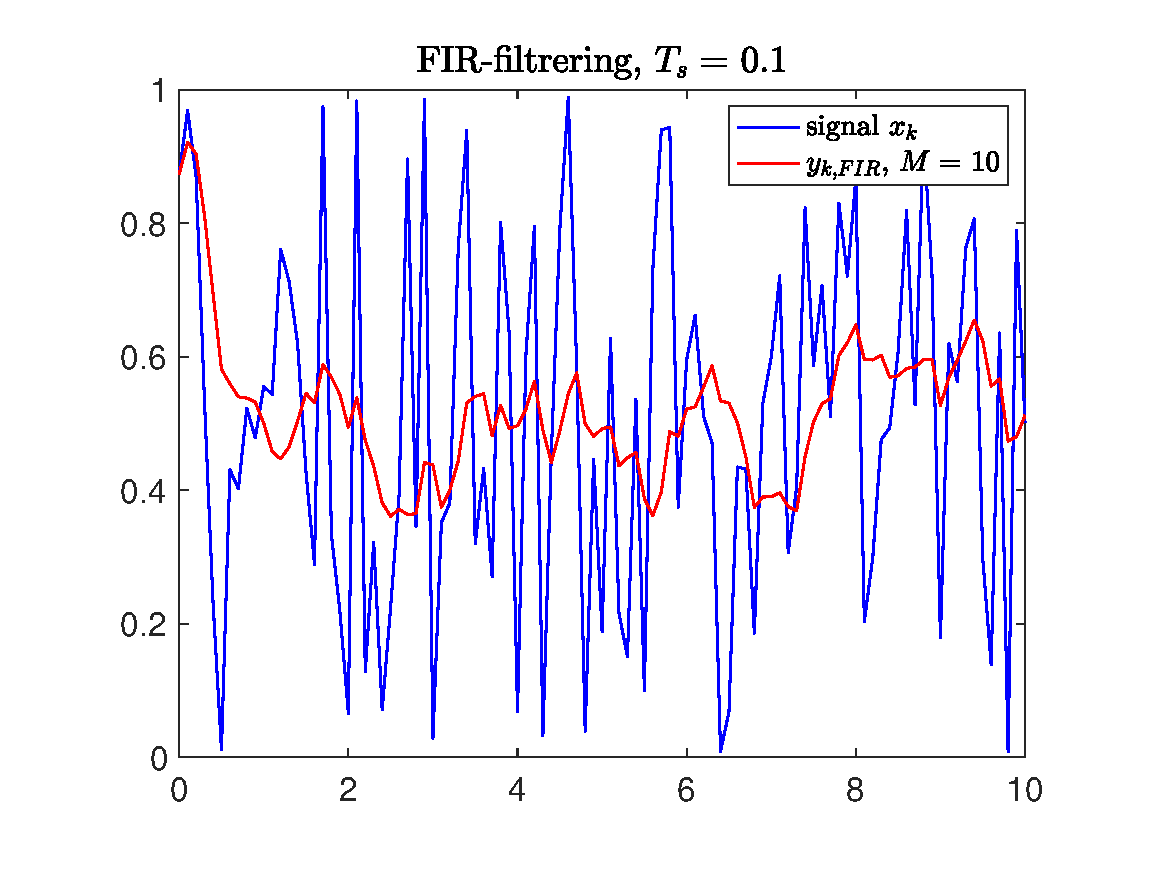
\includegraphics{3i.pdf}}
      \caption{Respons i FIR-filter med $M{=}10$. }
      \label{fig:3i}
    \end{figure}
    
    
\item Innholdet  i skallfilen \fbox{\tt FIR\_filter.m} er
  vist under, og som du ser benyttes beskrivende matematiske
  variabelnavn i  funksjonen. 

\begin{lstlisting}[caption={Skall for funksjonen for FIR-filtrering.},
 language= Matlab,   label=kode:FIR_funk,
numbers=none] 
function FilteredValue = FIR_filter(Measurement, NoOfMeas)

% juster på NoOfMeas her
% fyll inn filterkode

end
\end{lstlisting}
Ferdigstill koden i denne funksjonen. 
  Legg merke til at vi flytter 
  koden som justerer på $M$ inn i funksjonen. På den måten  blir mer
  funksjonen mer funskjonell i bruk, og $M$ kan spesifiseres 
  før  {\it for}-løkken i hovedfilen.
  

\item Vis at du får samme resultat som i figur~\ref{fig:3i} ved å
  endre {\it for}-løkken i skallfilen til
  
\begin{lstlisting}[caption={Syntaks for å kalle funksjonen {\tt FIR\_filter}.},
 language= Matlab,   label=kode:FIR_funk_kall,
numbers=none] 
M = 10;
for k = ..
    y_FIR(k) = FIR_filter(.., ..)
end
\end{lstlisting}

% Som du ser så sendes det inn målinger frem til og med
% indeks $k$, {\tt x(1:k)}. For å forstå hvorfor
% du må gjøre det på denne måten, prøv å send inn 
% alle målingene i {\tt x}  og se hva som  skjer, altså at kallet ser
% slik ut
% \fbox{\tt y\_FIR(k) = FIR\_filter(x, M)}. 

\subsubsection*{Effekten av $M$}
  
\item   For å teste betydningen av verdien på $M$ så
  er det i skallfilen {\tt oving3\_skallfil.m} laget til en egen
  seksjon som du kan kjøre direkte når du har laget ferdig funksjonen
  {\tt FIR\_filter}.  
  Vis at du får resultatet vist i  figur~\ref{fig:3i2}. 

    \begin{figure}[H]
      \centering
      \hspace*{0mm}\scalebox{0.5}{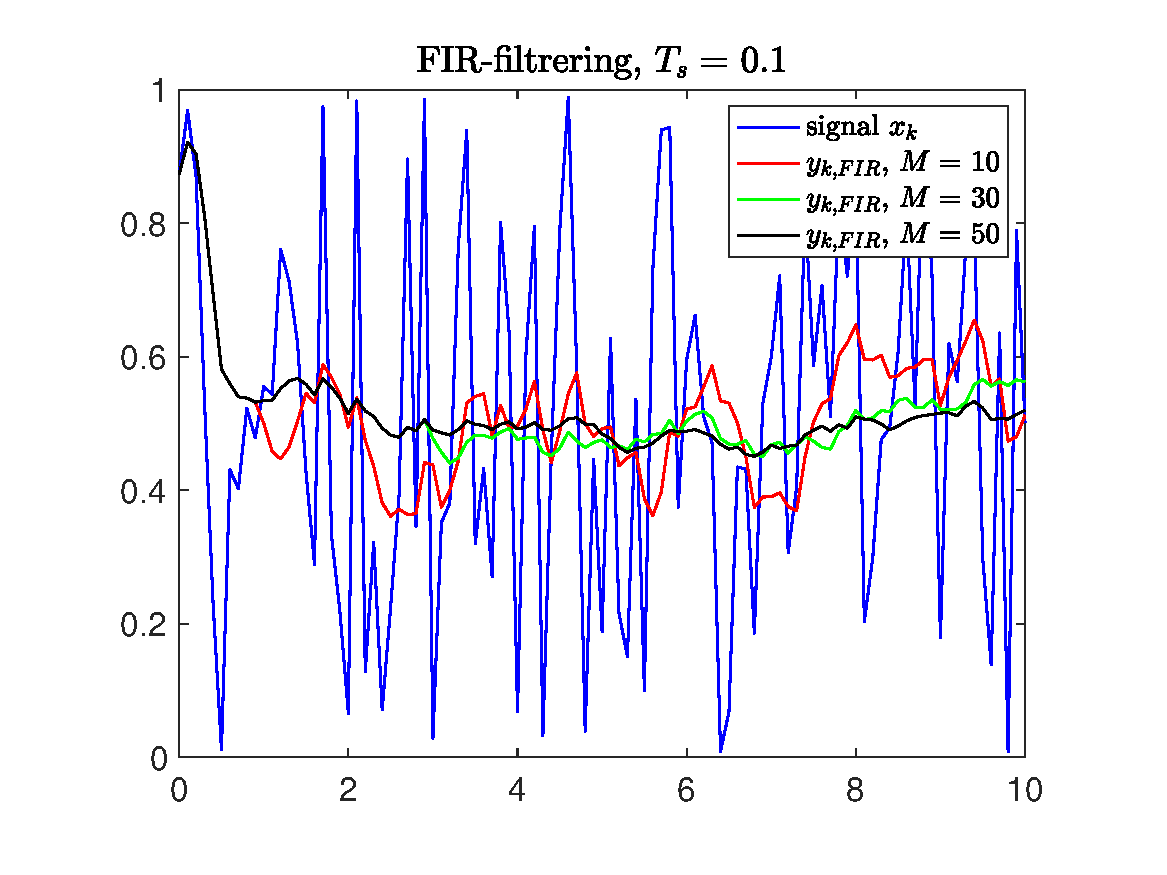
\includegraphics{3i2.pdf}}
      \caption{Respons i FIR-filter med $M{=}[10, 30, 50]$. }
      \label{fig:3i2}
    \end{figure}

    \item Hva er grunnen til at alle de tre filtrerte kurvene ligger over hverandre frem til
      ca 1 sekund? Samme fenomen ser du gjelder for 
      to av kurvene mellom 1 og 3 sekund. 

    \item  Er filtreringen som oppnås fornuftig i forhold til stigende
      tall på $M$? Begrunn svaret.

      \item Lek gjerne med andre verdier på $M$. Hva skjer hvis du
        setter \fbox{\tt M = k;} inne i {\it for}-løkken? 
\end{itemize}

  

  \begin{tcolorbox}[breakable, enhanced]
    \subsection*{Svar}
    
    
  \end{tcolorbox}




  
  % ********************************************************
  % oppgave j)
  % ********************************************************
  \newpage
    \runningheader{Oppgave j)}{}{Side \thepage\ av \numpages}
% ********************************************************
% oppgave j) 
% ******************************************************** 
\item
{\bf IIR-filter}

  I Lego-prosjektet skal du også jobbe med 
første ordens IIR-filter gitt som 
  \begin{equation}
  \label{eq:12}
 y_{k} = (1-\alpha)  {\cdot}y_{k-1} +  \alpha {\cdot}x_{k}
\end{equation}
hvor $0 {\leq} \alpha {\leq} 1$. Dette filteret bruker kun siste måling
$x_{k}$ som vektes med verdien $\alpha$, og legger sammen med forrige filtrerte
verdi $y_{k-1}$ som vektes med $(1{-}\alpha)$.  
Dersom $\alpha{=}1$ så har du ingen
filtrering og dersom $\alpha{=}0$ så får du en rett strek (alt
filtreres).

På samme måte som i deloppgave~\ref{oppg:i})  skal du også i denne
oppgaven først implementere kode for filteret gitt i
ligning~\eqref{eq:12} og deretter lage en egen funksjon av
IIR-filteret i skallfilen \fbox{\tt IIR\_filter.m}.

Ta utgangspunkt i koden i skallfilen hvor du ser at
målesignalet \fbox{\tt x} er det samme som i forrige
deloppgave, det samme gjelder samplingsfrekvensen og slutt-tiden.
Gjør følgende oppgaver: 

\begin{itemize}

\item  Implementer  kode for
IIR-filteret i ligning~\eqref{eq:12} i {\it for}-løkken. Kjør koden og
vis at du får resultatet vist i  figur~\ref{fig:3j}.
    \begin{figure}[H]
      \centering
      \hspace*{0mm}\scalebox{0.45}{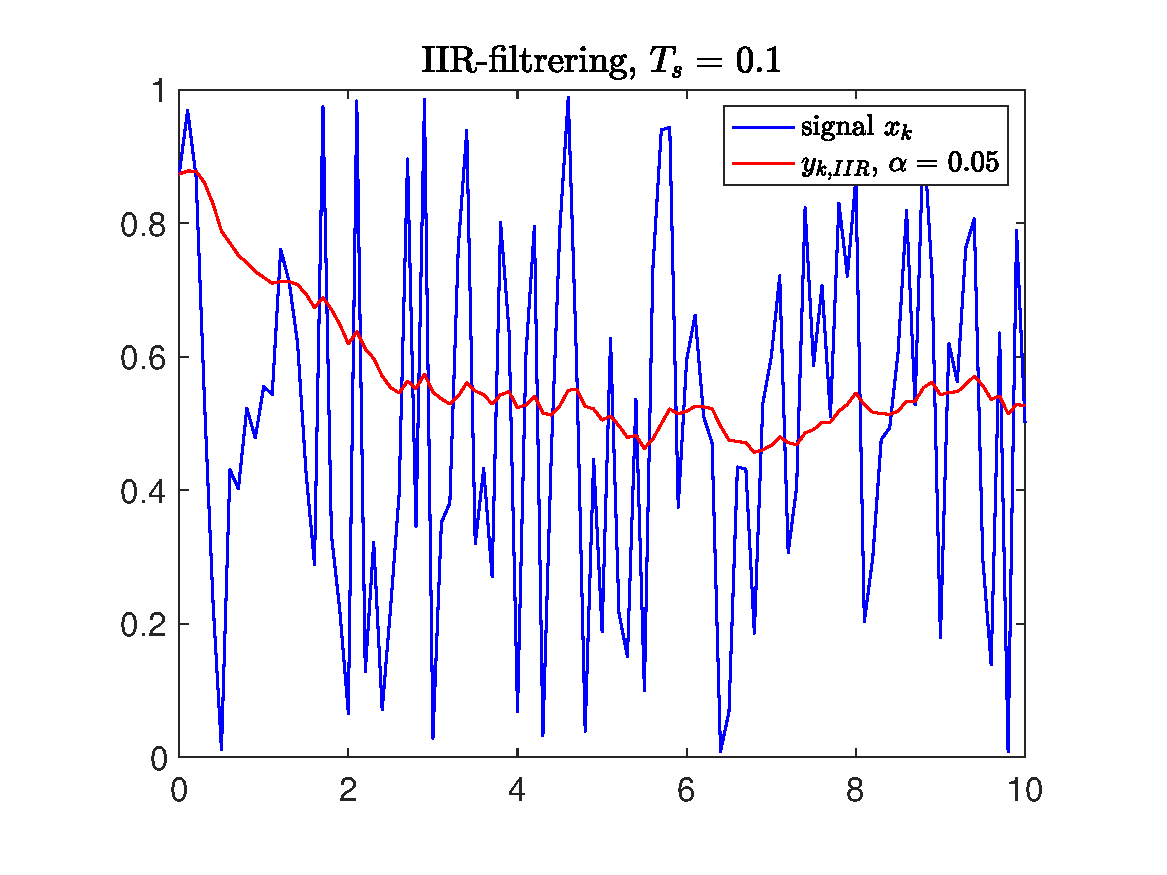
\includegraphics{3j.pdf}}
      \caption{Respons i IIR-filter med $\alpha{=}0.05$. }
      \label{fig:3j}
    \end{figure}
    
    
\item Innholdet i skallfilen \fbox{\tt IIR\_filter.m}  er vist under, 
og igjen brukes det beskrivende matematiske begrep for variabelnavn.

\begin{lstlisting}[caption={Skall for funksjonen for IIR-filtrering.},
 language= Matlab,   label=kode:IIR_funk, numbers=none, linewidth = 14.5cm] 
function FilteredValue = IIR_filter(OldFilteredValue, Measurement, para)
   % fyll inn
end
\end{lstlisting}
Ferdigstill koden i denne funksjonen.

\item Vis at du får samme   resultat som i figur~\ref{fig:3j} ved å
  endre {\it for}-løkken i skallfilen til 

\begin{lstlisting}[caption={Skall for funksjonen for IIR-filtrering.},
 language= Matlab,   label=kode:IIR_funk2,
 numbers=none]
 for k = 2:length(t)
    y_IIR(k) = IIR_filter(.., .., ..)
end
\end{lstlisting}

\subsubsection*{Effekten av $\alpha$}

\item For å teste betydningen av $\alpha$ så 
  er det i skallfilen {\tt oving3\_skallfil.m} laget til en egen
  seksjon som du kan kjøre direkte når du har laget ferdig funksjonen
  {\tt IIR\_filter}.    
Vis at du får resultatet vist i figur~\ref{fig:3j2}.

    \begin{figure}[H]
      \centering
      \hspace*{0mm}\scalebox{0.5}{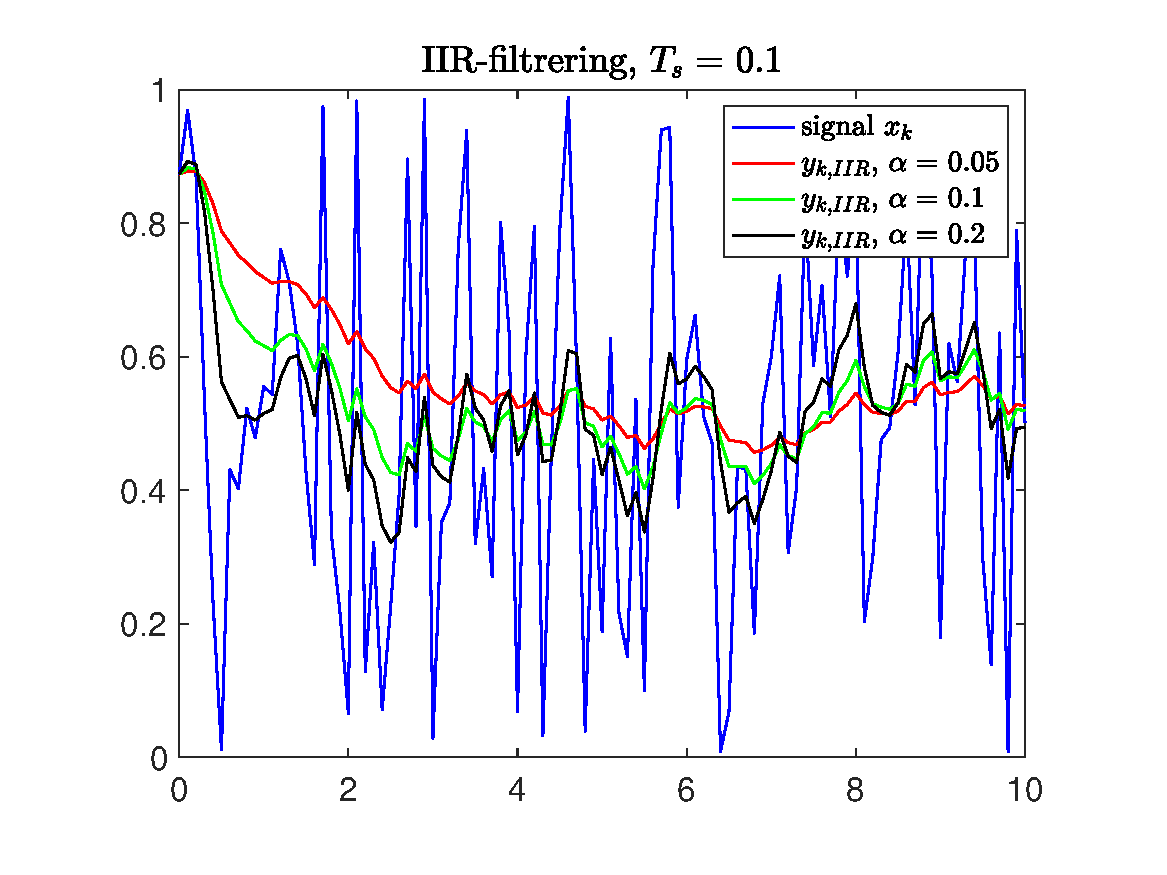
\includegraphics{3j2.pdf}}
      \caption{Respons i IIR-filter med $\alpha{=}[0.05, 0.1, 0.2]$. }
      \label{fig:3j2}
    \end{figure}

    \item   Er filtreringen som oppnås fornuftig i forhold til synkende tall på $\alpha$?

    \item Test ut $\alpha=0$ eller $\alpha=1$. Er
      resultatet fornuftig?

    \item Hva skjer dersom du setter $\alpha=-0.1$,  $\alpha=1.7$,
      $\alpha=2$ eller $\alpha=2.3$? Kan du forklare hva som skjer?

      
\end{itemize}
  

  \begin{tcolorbox}[breakable, enhanced]
    \subsection*{Svar}
    
    
  \end{tcolorbox}




  % ********************************************************
  % oppgave k)
  % ********************************************************
  \newpage
  \runningheader{Oppgave k), frivillig}{}{Side \thepage\ av \numpages}
% ********************************************************
% oppgave k) 
% ******************************************************** 
\item \label{pkt:FIR_IIR}
  {\bf Filtrering av ulike testsignal}
  
I denne oppgaven skal du bruke filterfunksjonene fra de forrige
deloppgavene til å  filtrere følgende fire testsignal (formulert tidskontinuerlig):
\begin{align}
\text{impuls:} \quad  x_{1}(t) & =
      \begin{cases}%
  0 &\text{for } t<10\\
  1 &\text{for } t=10\\
   0& \text{for } t >10
 \end{cases}\\
\text{firkantpuls:} \quad  x_{2}(t) & =
      \begin{cases}%
  0 &\text{for } t<10\\
  1 &\text{for } 10\leq t \leq 20\\
   0& \text{for } t > 20
 \end{cases}\\
\text{sinussignal:} \quad   x_{3}(t) & = 0.1 \sin(2\pi 0.1 t)+0.2 \label{eq:3}\\
  \text{sinussignal med støy:} \quad   x_{4}(t) &
                                                  = 0.1 \sin(2\pi 0.1 t)+0.2 +w(t)\label{eq:3a}  
\end{align}
I skallfilen
er den diskret tidsvektoren
\fbox{\tt t}  basert på en samplingsfrekvens på
  \begin{equation}
    \label{eq:1511}
      f_{s} = 2~\text{Hz}
    \end{equation}
    som gir en samplingstid på $T_{s}{=}0.5$ sekund.
    Siden Nyquistfrekvensen ved denne samplingsfrekvensen er
    \begin{equation}
      \label{eq:1_fs}
      f_{N}= 0.5{\cdot} f_{s} = 1~\text{Hz}
    \end{equation}
    så betyr det at vi sampler hurtig nok til å få med oss informasjonen fra
    sinussignalene gitt i ligningene~\eqref{eq:3} og \eqref{eq:3a},
    siden begge har en svingefrekvensen på $f{=}0.1$ Hz. 
    Videre er det i skallfilen gitt kode for de fire signalene
    \fbox{\tt x1} til  \fbox{\tt  x4} hvor bruker vi sammenhengen 
  \begin{equation}
    \label{eq:7}
    k{\cdot}T_{s} = t_{k}
  \end{equation}
  for å bestemme hvilken indeks $k$ som hører til et gitt tidspunkt.
  Siden vi jobber med Matlabindekser legger
  vi til 1 i beregningen. Dersom du velger et tidsskritt som ikke gir
  heltallsverdier av $k$, så må du bruke {\tt round}-funksjonen som
  \fbox{\tt k = round(t\_impuls/T\_s+1);}.

  Siden koden for FIR- og IIR-filteret er basert på variabelen {\tt x}, 
  og ikke {\tt x1}, {\tt x2}, {\tt x3} eller {\tt x4} som vi nettopp
  har definert, så velger du  hvilket signal du vil bruke der
  hvor det i skallfilen står:
  
\begin{lstlisting}[caption={Syntaks for å velge hvilket signal som
    skal filtreres.},  language= Matlab,   label=kode:velg,
numbers=none] 
%------------------------------------------------------
% Velg hvilket signal som skal filtreres. 
x = x1;
% For x1 og x2 er det smart å bruke kurveform = ':x';
% For x3 og x4 er det smart å bruke kurveform = '-';
kurveform = '-';
%------------------------------------------------------
\end{lstlisting}

  
Ferdigstill det som mangler i skallfilen, og gjør deretter følgende
oppgaver, hvor du for hver oppgave tar med resultatfigurene i innleveringen din.

\subsubsection*{\bf Filtrering av impulsen $x_{1}(t)$}

  Hensikten med dette signalet er
  å demonstrer hvorfor det heter FIR og IIR. Det betyr at du vil se at
  impulsen gir en  respons som blir 0 etter en viss tid for
  FIR-filteret ({\it finite}),  og en respons som aldri blir 0 for
  IIR-filteret ({\it infinite}). 

  \begin{itemize}
  \item Bruk \fbox{\tt M = 10}  og  \fbox{\tt alfa = 0.3} og kjør
    koden. Trykk inn på
    de røde og grønne linjene til hhv. FIR- og IIR-filteret rundt
    $t{\approx}30$ sekund og les av verdien. Ta med figuren i
    innleveringen din. 
  \item Er det logisk at maksimalverdien av  $y_{k,FIR}$  er 0.1 
    når \fbox{\tt M = 10}  mens maksimalverdien av   $y_{k,IIR}$ er 0.3 når
    \fbox{\tt alfa = 0.3}? Begrunn svaret.
  \end{itemize}

\subsubsection*{\bf Filtrering av firkantpulsen $x_{2}(t)$}

  Hensikten med dette signalet er å
  demonstrere {\it dynamikken} til filteret, altså hvor raskt det
  svinger seg inn til ny stasjonær verdi gitt at inngangen endres som
  et sprang. Husk at det positive spranget går ved
  $t_{\text{sprang}}{=}10$~sekund, og det negative spranget går ved
  $t_{\text{sprang}}{=}20$~sekund.
  
 
  \begin{itemize}
  \item Bruk \fbox{\tt M = 10}  og  \fbox{\tt alfa = 0.3} og kjør
    koden. Forklar med utgangspunkt i ligningen for FIR-filteret
    hvorfor responsen stiger som en lineær kurve før den
    til slutt flater ut.

  \item Bruk sammenhengen
    \begin{equation}
      M =\frac{t_{\text{FIR}}}{T_{s}}+ 1
    \end{equation}
    til å anslå filtervinduets lengde $t_{\text{FIR}}$~[s].  Hvordan
    relateres verdien av $t_{\text{FIR}}$ til responsen i FIR-filteret?
    
  \item Bruk sammenhengen
    \begin{equation}
  \label{eq:12ny}
  \boxed{\alpha = \frac{T_{s}}{\tau + T_{s}} }
\end{equation}
til å anslo  tidskonstanten $\tau$ for IIR-filteret. Hvordan
relateres verdien av $\tau$ til responsen i IIR-filteret?
   

  \item Hvordan endres dynamikken (hurtigheten) til IIR-filteret og
    selve responsen til FIR-filteret dersom du endrer til
    \fbox{\tt M = 15} og  \fbox{\tt alfa = 0.15}?

\end{itemize}

\newpage

\subsubsection*{\bf Filtrering av sinussignalet $x_{3}(t)$}

  Hensikten med dette signalet er å
  vise hvordan sinussignalet endres gjennom filteret, altså hvor mye
  amplituden blir redusert og hvor stor faseforskyvning er som
  funksjon av filterparametrene.   I denne oppgaven
  kan du med fordel endre kurveformen til \fbox{\tt '-'} slik 
  at kurvene blir ``renere''. 
 Gitt at resposnene i FIR- og IIR-filteret kan formuleres
    tidskontinuerlig som 
    \begin{align}
      \label{eq:11}
      y_{FIR}(t) & = Y_{FIR}{\cdot} \sin(2\pi f t + \varphi_{FIR}) \\
      y_{IIR}(t) & = Y_{IIR} {\cdot}\sin(2\pi f t + \varphi_{IIR}) 
    \end{align}

  \begin{itemize}
  \item  Bruk \fbox{\tt M = 15}  og  \fbox{\tt alfa = 0.15} og kjør
    koden. Hvor stor er amplitudene $Y_{FIR}$ og $Y_{IIR}$?
  \item Hvor stor er faseforskyvningen mellom
    innsignalet $x_{3}(t)$ og de to filtrerte signalene. Det vil si,
    bestem $\varphi_{FIR}^{\circ}$ og
    $\varphi_{IIR}^{\circ}$. (oppgitt i grader) 
  
  \item Øk samplingsfrekvensen $f_s$ til \fbox{\tt f\_s = 4}.
    Hvordan påvirker dette filtreringen? Hva er forklaringen
  på det som skjer? 
\item Behold \fbox{\tt f\_s = 4}. Hva må du gjøre med
  $M$ og $\alpha$ for å få et resultat som ligner på det du fikk når
  \fbox{\tt f\_s = 2}?
  
\item Sett \fbox{\tt M = k} inne i
  for-løkken, og forklar hva som skjer i FIR-filteret.


\end{itemize}

\subsubsection*{\bf Filtrering av sinussignalet med støy $x_{4}(t)$}
   Hensikten med dette signalet er å vise at hvordan
  du kan filtrere bort støyen og helst sitte igjen med sinussignalet som
  ligger i bunn.   

  \begin{itemize}
  \item 
  Behold \fbox{\tt f\_s = 4} og finn de $M$ og $\alpha$-verdiene som
  du synes fjerner støy på best mulig måte samtidig som selve
  sinussignalet beholdes i  størst mulig grad. Her er det ingen feil svar.
  \end{itemize}
  
  

  \begin{tcolorbox}[breakable, enhanced]
    \subsection*{Svar}
    
    
  \end{tcolorbox}



  
  % ********************************************************
  % oppgave l)
  % ********************************************************
  \newpage
  \runningheader{Oppgave l), frivillig}{}{Side \thepage\ av \numpages}
% ********************************************************
% oppgave l) 
% ******************************************************** 
\item
{\bf IIR-basert lavpass- og høypassfiltrering av {\it Chirp}-signal}

 I denne oppgaven skal vi ta utgangspunkt i sinussignalet fra
 ligning~\eqref{eq:3}  skrevet med tidsvarierende frekvens $f(t)$ som
\begin{align}
  x(t)  &= 0.1{\cdot}\sin\bigl(2 \pi f(t) {\cdot}t\bigr) + 0.2
\end{align}
Vi skal lage et  {\it chirp}-signal $x(t)$
som går fra $f_{\text{initial}}$~[Hz] til
$f_{\text{target}}$~[Hz] i løpet av 100 sekund.
Den tidsavhengige frekvensen $f(t)$ kan formuleres som
\begin{equation}
  \label{eq:1f}
  f(t) =
  f_{\text{initial}}+\Biggl(\frac{f_{\text{target}}-f_{\text{initial}}}{t_{\text{target}}}\Biggl)
  \cdot t
\end{equation}
hvor
\begin{itemize}
      \setlength\itemsep{0mm}
\item  $f_{\text{initial}}$ [Hz] tilsvarer startfrekvensen 
\item  $f_{\text{target}}$ [Hz] tilsvarer sluttfrekvensen
\item  $t_{\text{target}}$ [s] er tidspunktet når frekvensen er
  $f_{\text{target}}$ 
\end{itemize}

Du skal bruke to forskjellige varianter av første ordens IIR-filter, nemlig
  \begin{align}
 y_{k} &= (1-\alpha)  {\cdot}y_{k-1} +  \alpha {\cdot}x_{k}\label{eq:lavpass}\\
 y_{k} &= a_{1}  {\cdot}y_{k-1} +  b_{0}{\cdot}x_{k} + b_{1}{\cdot}x_{k-1}\label{eq:hoypass}
\end{align}
Du kjenner godt til den første varianten i ligning~\eqref{eq:lavpass} som egentlig er et
{\it lavpassfilter}. Det betyr at lave frekvenser passerer gjennom, mens høye frekvenser
stoppes i filteret.

Filteret i ligning~\eqref{eq:hoypass} er et filter som kan
fjerne DC-ledd (konstantledd), og er dermed et såkalt {\it
  høypassfilter}. Lave frekvenser, som egentlig kan betraktes som et
langsomtvarierende konstantledd fjernes og høye frekvenser slippes
gjennom. Ved å velge like verdier for 
$b_{0}$ og $b_{1}$, men med motsatt fortegn, så filtreres faktisk
DC-leddet helt bort!
Ferdigstill og kjør koden i skallfilen. Ta med figuren i innleveringen din.

  

  \begin{tcolorbox}[breakable, enhanced]
    \subsection*{Svar}
    
    
  \end{tcolorbox}



  % ********************************************************
  % oppgave m)
  % ********************************************************
  \newpage
  \runningheader{Oppgave m), frivillig}{}{Side \thepage\ av \numpages}
% ********************************************************
% oppgave m) 
% ********************************************************  
\item
  {\bf Kodebasert filtrering i {\tt MATLAB Function}-blokk i Simulink}

  Sinusfunksjonen $x(t)$ i ligning~\eqref{eq:3}
  oppgave~\ref{pkt:FIR_IIR}) kan skrives som 
\begin{equation}
  x(t) = 0.1 \sin(0.628t)+0.2, \quad \forall \quad 0<t<30 \label{eq:3_w}
\end{equation}

Åpne Simulink-skallfilen \fbox{\tt oving3\_a\_m\_skallfil.slx}, og gå videre
til subsystemet \fbox{\tt Oppgave 3m)}. 
Der ser du at sinusfunksjonen i ligning~\eqref{eq:3_w} allerede er implementert.
Siden vi ikke har noen integrator i
modellen er valget av numerisk løser ikke så viktig. Velg derfor bare
{\it Eulers forovermetode} med tidsskritt   $T_{s}{=}0.5$, som tilsvarer
en samplingsfrekvens   på $f_{s}{=}2$~Hz på samme måte som
utgangspunktet i  oppgave~\ref{pkt:FIR_IIR}).
 
\begin{itemize}
\item  I \fbox{\tt  MATLAB  Function}-blokken skal du implementere
  IIR-filteret gitt som
  \begin{equation}
    y(k) = (1-\alpha)  {\cdot}y(k-1) +  \alpha {\cdot}x(k) \tag{\ref{eq:12}}
  \end{equation}
  med \fbox{\tt alfa = 0.15}. 
  For å gjøre et indeksskift $y(k)$ til $y(k-1)$ så benyttes
  en \fbox{\tt Memory}-blokk fra {\tt Discrete}-mappen. Denne
  forsinker signalet med ett tidsskritt før det mates inn som et
  inngangssignal.  Husk å spesifisere riktig
  {\tt Initial condition} for {\tt Memory}-blokken.

  Simuler i 30 sekund, og vis at du får et
  resultat som er identisk med det du fikk i oppgave~\ref{pkt:FIR_IIR}).

\end{itemize}
  

  \begin{tcolorbox}[breakable, enhanced]
    \subsection*{Svar}
    
    
  \end{tcolorbox}


  

  % ********************************************************
  % oppgave n)
  % ********************************************************
  \newpage
  \runningheader{Oppgave n), frivillig}{}{Side \thepage\ av \numpages}

% ********************************************************
% oppgave n) 
% ******************************************************** 
\item
    {\bf Demonstrasjon av sampling og nedfolding}

  I denne oppgaven skal du ikke programmere noe, men du kan kjøre
  koden og leke litt med den høyeste frekvensen $f$ på det analoge
  signalet som
  skal samples, og samtidig bestemme hvilken samplingsfrekvens du vil bruke. Koden
  kan brukes til å demonstrere nedfolding, og du får følelsen av å
  observere dette i sann tid.  Det diskret målesignalet $y_{k}$ er
  basert på måling av det kontinuerlige ``analoge'' signal $y(t)$.

Som innlevering kan du ta med de signalene du har lekt med og samtidig
forklare hva som skjer.



  

  \begin{tcolorbox}[breakable, enhanced]
    \subsection*{Svar}
    
    
  \end{tcolorbox}


  
  % ********************************************************
  % oppgave o)
  % ********************************************************
  \newpage
  \runningheader{Oppgave o), frivillig}{}{Side \thepage\ av \numpages}

% ********************************************************
% oppgave o) 
% ******************************************************** 
\item   {\bf Demonstrasjon av oppsampling}

  Oppsampling  (eng: {\it upsamling}) er en teknikk for å rekonstruere
  samplede signaler.   I denne
  oppgaven skal vi demonstrere dette for en tenkt problemstilling hvor
  du har en motor med en såkalt encoder som kan måle vinkelposisjonen
  til motoren. Anta
  at motoren roterer ca.\ 10 runder, og at du sampler
  vinkelposisjonen for hver {\tt delta\_phi=260}$^{\circ}$, og at
  dette skjer med et 
  tidsskrittet på {\tt T\_s=0.2}~sekund. Dette gir en vinkelhastighet på
  \begin{equation}
\omega_{d} = \frac{260^{\circ}}{0.2}= 1300^{\circ}/\text{s}    
\end{equation}
hvor subskript $d$ impliserer ``degrees''. 
Ved å beregne og plotte
  \begin{equation}
y(t) = \sin(\omega_{d}{\cdot} t)    
  \end{equation}
så kan du  få et visuelt bilde på rotasjonen som har
foregått.  Vær klar over at sinus-funksjonen forventer
en vinkel oppgitt i radianer og ikke grader som over, og at vi strengt
tatt burde skrevet
  \begin{equation}
y(t) = \sin\Bigl(\omega_{d}{\cdot} t {\cdot} \frac{2\pi}{360} \Bigl)    
  \end{equation}
Når det er sagt, så har Matlab en  {\tt sind()}-funksjon som tar
grader som argument.


Som du vil se fra kurven øverst til høyre når du kjører koden,
så er problemet at vi sampler såpass sjelden at det ser ut 
som motoren kun har rotert et par runder. Etter at du trykker OK, vil
de se at vi legger     
inn fiktive, men egentlig høyst reelle, vinkelmålinger og tidspunkt
mellom de samplede  målingene. På den måten utvider vi datasettet
vårt, og grunnen til at vi vet at dette går fint er at motoren har
rotert jevnt i én retning. 

Matlabfunksjonen for å oppsample er
\fbox{\tt interp} som interpolerer 
verdier mellom de avleste vinkelposisjonsmålingene.

Lek gjerne med verdien på {\tt delta\_phi}, fra 30$^{\circ}$ og
oppover. Ved hvilken verdi går det galt?

Som innlevering kan du ta med de signalene du har lekt med og samtidig
forklare hva som skjer.
  

  \begin{tcolorbox}[breakable, enhanced]
    \subsection*{Svar}
    
    
  \end{tcolorbox}


\end{enumerate}


\end{document}









